%%%%%%%%%%%%%%%%%%%%%%%%%%%%%%%%%%%%%%%%%
% Jacobs Landscape Poster
% LaTeX Template
% Version 1.1 (14/06/14)
%
% Created by:
% Computational Physics and Biophysics Group, Jacobs University
% https://teamwork.jacobs-university.de:8443/confluence/display/CoPandBiG/LaTeX+Poster
% 
% Further modified by:
% Nathaniel Johnston (nathaniel@njohnston.ca)
%
% This template has been downloaded from:
% http://www.LaTeXTemplates.com
%
% License:
% CC BY-NC-SA 3.0 (http://creativecommons.org/licenses/by-nc-sa/3.0/)
%
%%%%%%%%%%%%%%%%%%%%%%%%%%%%%%%%%%%%%%%%%

%----------------------------------------------------------------------------------------
%	PACKAGES AND OTHER DOCUMENT CONFIGURATIONS
%----------------------------------------------------------------------------------------

\documentclass[final]{beamer}

\usepackage[scale=1.24]{beamerposter} % Use the beamerposter package for laying out the poster
\usepackage[utf8]{inputenc}
\usepackage[T1]{fontenc}
\usepackage[francais]{babel}
\usepackage{pgf,tikz}
\usetikzlibrary{arrows}
\usepackage{graphicx}
\usepackage{filecontents} 
\usepackage{mathrsfs}
\usepackage{amsthm}
\usepackage{amssymb}
\definecolor{wwqqtt}{rgb}{0.4,0,0.2}
\definecolor{zzttqq}{rgb}{0.6,0.2,0}
\definecolor{uququq}{rgb}{0.25,0.25,0.25}
\definecolor{qqqqff}{rgb}{0,0,1}
\definecolor{dcrutc}{rgb}{0.86,0.08,0.24}
\definecolor{qqwuqq}{rgb}{0,0.39,0}
\definecolor{cqcqcq}{rgb}{0.75,0.75,0.75}

\def\restriction#1#2{\mathchoice
              {\setbox1\hbox{${\displaystyle #1}_{\scriptstyle #2}$}
              \restrictionaux{#1}{#2}}
              {\setbox1\hbox{${\textstyle #1}_{\scriptstyle #2}$}
              \restrictionaux{#1}{#2}}
              {\setbox1\hbox{${\scriptstyle #1}_{\scriptscriptstyle #2}$}
              \restrictionaux{#1}{#2}}
              {\setbox1\hbox{${\scriptscriptstyle #1}_{\scriptscriptstyle #2}$}
              \restrictionaux{#1}{#2}}}
\def\restrictionaux#1#2{{#1\,\smash{\vrule height .8\ht1 depth .85\dp1}}_{\,#2}}

\usetheme{confposter} % Use the confposter theme supplied with this template

\setbeamercolor{block title}{fg=ngreen,bg=white} % Colors of the block titles
\setbeamercolor{block body}{fg=black,bg=white} % Colors of the body of blocks
\setbeamercolor{block alerted title}{fg=white,bg=dblue!70} % Colors of the highlighted block titles
\setbeamercolor{block alerted body}{fg=black,bg=dblue!10} % Colors of the body of highlighted blocks
% Many more colors are available for use in beamerthemeconfposter.sty

%-----------------------------------------------------------
% Define the column widths and overall poster size
% To set effective sepwid, onecolwid and twocolwid values, first choose how many columns you want and how much separation you want between columns
% In this template, the separation width chosen is 0.024 of the paper width and a 4-column layout
% onecolwid should therefore be (1-(# of columns+1)*sepwid)/# of columns e.g. (1-(4+1)*0.024)/4 = 0.22
% Set twocolwid to be (2*onecolwid)+sepwid = 0.464
% Set threecolwid to be (3*onecolwid)+2*sepwid = 0.708

\newlength{\sepwid}
\newlength{\onecolwid}
\newlength{\twocolwid}
\newlength{\threecolwid}
\setlength{\paperwidth}{48in} % A0 width: 46.8in
\setlength{\paperheight}{36in} % A0 height: 33.1in
\setlength{\sepwid}{0.024\paperwidth} % Separation width (white space) between columns
\setlength{\onecolwid}{0.22\paperwidth} % Width of one column
\setlength{\twocolwid}{0.464\paperwidth} % Width of two columns
\setlength{\threecolwid}{0.708\paperwidth} % Width of three columns
\setlength{\topmargin}{-0.5in} % Reduce the top margin size
%-----------------------------------------------------------

\usepackage{graphicx}  % Required for including images

\usepackage{booktabs} % Top and bottom rules for tables

%----------------------------------------------------------------------------------------
%	TITLE SECTION 
%----------------------------------------------------------------------------------------

\title{Approximation de Surface $C^k$-régulière à partir de Patchs de Surface} % Poster title

\author{Christian Gout, Alexandre Vieira \& Conrad Hillairet} % Author(s)

\institute{INSA de Rouen - Université de Rouen} % Institution(s)


%----------------------------------------------------------------------------------------

\begin{document}

\addtobeamertemplate{block end}{}{\vspace*{2ex}} % White space under blocks
\addtobeamertemplate{block alerted end}{}{\vspace*{2ex}} % White space under highlighted (alert) blocks

\setlength{\belowcaptionskip}{2ex} % White space under figures
\setlength\belowdisplayshortskip{2ex} % White space under equations

\begin{frame}[t] % The whole poster is enclosed in one beamer frame

\begin{columns}[t] % The whole poster consists of three major columns, the second of which is split into two columns twice - the [t] option aligns each column's content to the top

\begin{column}{\sepwid}\end{column} % Empty spacer column

\begin{column}{\onecolwid} % The first column

%----------------------------------------------------------------------------------------
%	OBJECTIVES
%----------------------------------------------------------------------------------------

\begin{alertblock}{Objectifs}

A partir d'un ensemble fini de patchs de surface donnés, il s'agit:
\begin{itemize}
\item De constuire une approximation régulière approchant la surface sur ces patchs
\item Cet approximant sera une spline polynomiale par morceaux 
\item De tenir compte de l'aspect continu des données  
\item D'estimer les erreurs et d'implémenter numériquement l'approximant
\end{itemize}

\end{alertblock}

%----------------------------------------------------------------------------------------
%	INTRODUCTION
%----------------------------------------------------------------------------------------

\begin{block}{Introduction}
Les méthodes usuelles se contentent de prendre des points sur les patchs: on a alors des 
données de Lagrange. A l'inverse de ces méthodes, on veut ici tenir compte de l'aspect continu des données, prendre en compte leur aspect originel, en particulier leur régularité.\\

A ces fins, on introduit \textbf{un critère de fidélité aux données} sous la forme d'une norme $L^2(\Omega)$.\\

On considère que l'on connaît initialement :
\begin{itemize}
\item $\Omega$ : un ouvert connexe borné non vide de $\mathbb{R}^n$ à forntière lipschitzienne (en pratique $n$=2)
\item une famille finie d'ouverts de $\Omega$ : $(\omega_j)^N_{j=1} \subset \mathcal{P}(\Omega)$
\item une fonction $f$ définie sur $\Omega$, donnée sur $\omega = \cup_{j=1}^N\omega_j$ et inconnue sur $\Omega \backslash \omega$.
\end{itemize}
	
%This statement requires citation \cite{Smith:2012qr}.

\end{block}

%------------------------------------------------

\begin{figure}
%\includegraphics[width=1.0\linewidth]{fig.png}
\input{myfig.tikz}
\caption{Exemple de trois patchs à partir desquels on veut reconstruire $f$ sur $\Omega$}
\label{fig1}
\end{figure}

%----------------------------------------------------------------------------------------

\end{column} % End of the first column

\begin{column}{\sepwid}\end{column} % Empty spacer column

\begin{column}{\twocolwid} % Begin a column which is two columns wide (column 2)

\begin{columns}[t,totalwidth=\twocolwid] % Split up the two columns wide column

\begin{column}{\onecolwid}\vspace{-.6in} % The first column within column 2 (column 2.1)

%----------------------------------------------------------------------------------------
%	
%----------------------------------------------------------------------------------------
\begin{block}{}
\textbf{But} : Construire une fonction régulière $\phi$ sur $\Omega$ approximant $f$ sur $\omega$.\\

On émet les hypothèses suivantes:
\begin{enumerate}
\item $f \in \mathcal{H}^m(\Omega)$
\item $\phi \in \mathcal{H}^m(\Omega) \cap C^k(\overline{\Omega}) , k \in \mathbb{N} , m > \frac{n}{2}$
\end{enumerate}

Si $m>k+\frac{n}{2}$ , le problème d'interpolation $\phi|_{\omega}=f|_{\omega}$ admet une infinité de solution. La théorie de Duchon \cite{Duchon76} nous permet d'en obtenir une. Mais la taille considérable des systèmes à résoudre nous pousse vers une autre solution.\\

Nous considérons $\mathcal{K}=\{v\in\mathcal{H}^m(\Omega),v|_{\omega}=f|_{\omega}\}$ convexe. Le problème d'interpolation devient:
\begin{center}
Trouver $\sigma \in \mathcal{K}$ : 
\begin{equation}
\forall v \in \mathcal{K} , |\sigma|_{m,\Omega} \leq |v|_{m,\Omega}
\label{eq1}
\end{equation}
où $|\sigma|_{m,\Omega} = \sqrt{\sum_{|\alpha|=m}{\int_{\Omega}{(\partial^{\alpha}{v(x)})^2}}}$
\end{center}

L'existence et l'unicité de (\ref{eq1}) ont été montrées dans \cite{gout97etude}. On a l'équivalence des normes dans $\mathcal{H}^m(\Omega)$ :
\begin{enumerate} 
\item $||u||_{m,\Omega} = \sqrt{\sum_{|\alpha|=\leq m}{\int_{\Omega}{(\partial^{\alpha}{v(x)})^2}}}$
\item  $|||u|||=\sqrt{||u||^2_{0,\omega} + |u|_{m,\Omega}^2}$ , où $||u||^2_{0,\omega}= \sum_{j=1}^{N}{\int_{\omega_j}{v^2(x)dx}}$ 
\end{enumerate}

$\sigma$ solution de (\ref{eq1}), est l'unique élément de norme $|||.|||$ minimale. Mais il est impossible de vérifier en dimension finie 
un nombre infini de conditions d'interpolation, on ne peut donc pas construire $\sigma$ par discrétisation de (\ref{eq1}). Pour prendre en compte cet aspect continu des données $\restriction{f}{\omega}$ on choisit $\phi$ non plus comme une surface d'interpolation, mais d'ajustement.\\

On va donc construire une $D^m$-spline régulière \cite{arcang89Applic} qui sera discrétisée dans un espace polynomial par morceaux. On introduit pour cela la fonctionnelle : $\mathcal{J}_{\varepsilon}$ sur $\mathcal{H}^m(\Omega)$:
\[ \mathcal{J}_{\varepsilon}(v) = ||v-f||_{0,\omega}^2 + \varepsilon|v|^2_{m,\Omega} \]
$ ||v-f||_{0,\omega}^2 $ est le critère de fidélité aux données et honore l'aspect continu de celles-ci; $\varepsilon > 0 $ est un paramètre de régularité.\\

\end{block}

%----------------------------------------------------------------------------------------

\end{column} % End of column 2.1

\begin{column}{\onecolwid}\vspace{-.6in} % The second column within column 2 (column 2.2)

%----------------------------------------------------------------------------------------
%	METHODS
%----------------------------------------------------------------------------------------
\begin{block}{Approximation de $||.||_{0,\omega}$}
On veut donner une formule de quadrature pour approximer $||.||_{0,\omega}$ à un certain ordre. On introduit pour cela:
\begin{itemize}
\item Des noeuds d'intégration : \item $\forall \eta \in E \subset \mathbb{R}^+_* , \forall 1\leq j\leq N , (\xi_i)_{i=1}^{L(\eta,j)}$  points distincts de $\overline{\omega_j}$
\item Des coefficients d'intégration : $(\lambda_i)_{i=1}^{L(\eta,j)} \subset \mathbb{R}_*^+$
\item $\forall \eta \in E, \forall 1\leq j \leq N, \forall v \in C^0(\overline{\omega_j}), \ell^{\eta}_j(v) = \sum_{i=1}^L{\lambda_iv(\xi_i)}$
\item $\forall \eta \in E, \forall v \in C^0(\overline{\omega_j}), \ell^{\eta}(v) = \sum_{j=1}^N{\ell_j^{\eta}(v)}$
\end{itemize}
Si $\exists c,t >0, \forall \eta \in E , \forall v \in \mathcal{H}^m(\Omega),\forall 1 \leq j \leq N , | \ell^{\eta}_j(v^2) - \int_{\omega_j}{v^2dx}| \leq c\eta^t||v||^2_{m,\Omega}$ 
, Alors on a la formule d'intégration numérique abstraite pour $||.||_{0,\omega}^2 \approx \ell^{\eta}(v^2)$. Pour avoir la convergence quand $\eta\to  0$, les noeuds doivent vérifier : $\max_{1 \leq i \leq L}{\min_{1 \leq k \leq L , k \neq i}{\delta(\xi_i,\xi_k)}}\leq \eta$ (répartition uniforme des noeuds).
\end{block}

\begin{block}{Méthodes}
\begin{enumerate}
\item Le critère de fidélité aux données aurait pu être sous la forme d'une norme de $L^1(\Omega)$;
en minimisant alors le volume entre l'approximante : $\phi$ et $f$ sur $\omega$.
Sa non-hilbertianité, fait donc pencher le choix de la norme du critère vers celle de $L^2(\Omega)$.
\item En pratique, si on a une triangulation $\tau_n$ de $\omega$, de n-simplexes $\tau$ de diamètre inférieur ou égal à $\eta$, et que $(a_i)_{i=1}^3 ,(b_i)_{i=1}^3$ et $c$ sont respectivement les sommets, milieux et barycentre de chaque $\tau$, alors on utilise la formule $\mathcal{P}_3$ : $\ell^{\eta}(v) = \sum_{\tau \in \tau_n}{meas(T)[\frac{1}{20}\sum_{i=1}^3{v(a_i)}+\frac{2}{15}\sum_{i=1}^3{v(b_i)}+\frac{9}{20}v(c)]}$
\end{enumerate}
\end{block}
\begin{figure}[!h]
\centering
\begin{tikzpicture}[line cap=round,line join=round,>=triangle 45,x=1.0cm,y=1.0cm]
\clip(3.82,-7.67) rectangle (20.82,1.26);
\fill[color=zzttqq,fill=zzttqq,fill opacity=0.1] (3.9,1.17) -- (20.66,1.21) -- (20.72,-7.55) -- (3.9,-7.53) -- cycle;
\fill[line width=2.4pt,color=zzttqq,fill=zzttqq,fill opacity=0.1] (7.74,-1.31) -- (7.74,0.38) -- (16.27,0.42) -- (16.29,-1.3) -- (18.12,-1.3) -- (18.2,-5.94) -- (6.68,-6.03) -- (6.68,-4.49) -- (5.62,-4.5) -- (5.62,-1.31) -- cycle;
\draw [line width=1.1pt, rotate around={1.21:(11.9,-3.14)}] (11.9,-3.14) ellipse (5.48cm and 2.78cm);
\draw [color=wwqqtt] (3.9,1.17)-- (20.66,1.21);
\draw [color=wwqqtt] (20.66,1.21)-- (20.72,-7.55);
\draw [color=wwqqtt] (20.72,-7.55)-- (3.9,-7.53);
\draw [color=wwqqtt] (3.9,-7.53)-- (3.9,1.17);
\draw (3.9,0.37)-- (20.67,0.45);
\draw (20.68,-1.29)-- (3.9,-1.31);
\draw (3.9,-3.05)-- (20.69,-3.12);
\draw (20.7,-4.39)-- (3.9,-4.51);
\draw (3.9,-6.05)-- (20.71,-5.91);
\draw (3.9,-6.55)-- (20.72,-6.39);
\draw (5.62,1.17)-- (5.62,-7.54);
\draw (6.68,-7.54)-- (6.68,1.17);
\draw (7.74,1.17)-- (7.75,-7.54);
\draw (8.98,-7.54)-- (8.96,1.18);
\draw (10.78,1.18)-- (10.78,-7.54);
\draw (12.9,-7.55)-- (12.82,1.19);
\draw (14.62,1.19)-- (14.7,-7.55);
\draw (16.34,-7.55)-- (16.26,1.19);
\draw (18.08,1.2)-- (18.22,-7.55);
\draw (19.78,-7.55)-- (19.68,1.2);
\draw [line width=2.4pt,color=zzttqq] (7.74,-1.31)-- (7.74,0.38);
\draw [line width=2.4pt,color=zzttqq] (7.74,0.38)-- (16.27,0.42);
\draw [line width=2.4pt,color=zzttqq] (16.27,0.42)-- (16.29,-1.3);
\draw [line width=2.4pt,color=zzttqq] (16.29,-1.3)-- (18.12,-1.3);
\draw [line width=2.4pt,color=zzttqq] (18.12,-1.3)-- (18.2,-5.94);
\draw [line width=2.4pt,color=zzttqq] (18.2,-5.94)-- (6.68,-6.03);
\draw [line width=2.4pt,color=zzttqq] (6.68,-6.03)-- (6.68,-4.49);
\draw [line width=2.4pt,color=zzttqq] (6.68,-4.49)-- (5.62,-4.5);
\draw [line width=2.4pt,color=zzttqq] (5.62,-4.5)-- (5.62,-1.31);
\draw [line width=2.4pt,color=zzttqq] (5.62,-1.31)-- (7.74,-1.31);
\begin{scriptsize}
\draw (14,-2) node {\large{$\Omega$}};
\draw (17.5,-5) node{\large{$\Omega_h$}};
\draw (19,-6) node{\large{$\tilde{\Omega}$}};
\end{scriptsize}
\end{tikzpicture}
\caption{Définition des ensembles $\Omega$, $\tilde{\Omega}$ et $\Omega_h$ }
\label{fig2}
\end{figure}


%----------------------------------------------------------------------------------------

\end{column} % End of column 2.2

\end{columns} % End of the split of column 2 - any content after this will now take up 2 columns width

\end{column} % End of the second column

\begin{column}{\sepwid}\end{column} % Empty spacer column

\begin{column}{\onecolwid} % The third column

%----------------------------------------------------------------------------------------
%	Approimation Dm-Splines
%----------------------------------------------------------------------------------------

\begin{block}{Approximation par $D^m$-spline}
Soient $H$ un sous-espace borné de $\mathbb{R}^+\backslash\{0\}$ pour lequel $0$ est un point d'accumulation, $\tilde{\Omega}$ un polygone ouvert de $\mathbb{R}^n$ tel que $\Omega\subset\tilde{\Omega}$ et, pour tout $h\in H$, on note $\tilde{\mathscr{T}}_h$ une triangulation sur $\tilde{\Omega}$ au moyen d'éléments $K$ dont le diamètre $h_K$ sont inférieurs ou égal à $h$ et soit $\tilde{V}_h$ un espace d'éléments finis construit sur $\tilde{\mathscr{T}}_h$ tel que : $\tilde{V}_h$ est un sous-espace de dimension fini de $H^m\left(\tilde{\Omega}\right)\cap C^k\left(\overline{\tilde{\Omega}}\right)$ (voir fig. \ref{fig2})\\
De plus, pour étudier la convergence de l'approximation, on suppose qu'il existe une famille d'opérateurs linéaires continus $(\tilde{\Pi}_h)_{h\in H}$ de $H^m(\Omega)$ dans $\tilde{V}_h$ satisfaisant :
	\[\exists C>0;\ \forall h\in H,\ \forall l=0,...,m-1,\ \forall v\in H^m(\tilde{\Omega})\]
\begin{equation} \label{eq6.1}
\left| v-\tilde{\Pi}_h v\right|_{l,\tilde{\Omega}}\leq Ch^{m-1}|v|_{m,\tilde{\Omega}}
\end{equation}
\begin{equation} \label{eq6.2}
	\forall v\in H^m(\tilde{\Omega}), \lim_{h\to 0} \left|v-\tilde{\Pi}_h v \right|_{m,\tilde{\Omega}}=0
\end{equation}
On admet une certaine régularité sur $\tilde{\mathscr{T}}_h$ (voir famille régulière dans \cite{ciarlet72gal}). On construit $\Omega_h$ comme l'union des rectangles $K$ dont l'intersection avec $\Omega$ est non vide (voir fig. \ref{fig2}) qui vérifie : 
\begin{eqnarray}
	\label{eq9} \forall h\in H, \Omega\subset\Omega_h\subset\tilde{\Omega}\\
	\label{eq10} \lim_{h\to 0} \mu(\Omega_h\backslash\overline{\Omega})=0
\end{eqnarray}
Ainsi, on définit :
	\begin{equation}\label{eq11} V_h=\{\restriction{\phi}{\Omega_h}| \phi\in\tilde{V}_h\}\end{equation}
Pour tout $\varepsilon>0$, on considère le problème de minimisation suivant : trouver $\sigma_{\varepsilon,h}^\eta\in V_h$ satisfaisant :
	\begin{equation} \label{eq12} \forall v_h\in V_h,\ J_{\varepsilon, h}^\eta (\sigma_{\varepsilon, h}^\eta)\leq J_{\varepsilon, h}^\eta (v_h) \end{equation}
où $J_{\varepsilon, h}^\eta$ est la fonctionnelle définie par :
	\[J_{\varepsilon, h}^\eta=\ell^\eta \left[(v_h-f)^2\right]+\varepsilon |v_h|^2_{m,\Omega_h}\]
On considère ensuite le problème variationnel suivant : trouver $\sigma_{\varepsilon,h}^\eta\in V_h$ satisfaisant :
	\begin{equation} \label{eq13} \forall v_h\in V_h,\ \ell^\eta (\sigma_{\varepsilon, h}^\eta v_h)+ \varepsilon \left(\sigma_{\varepsilon, h}^\eta,v_h\right)=\ell^\eta(fv_h) \end{equation}
où $(u,v)_{m,\Omega_h}=\sum_{|\alpha|=m} \int_{\Omega_h} \partial^\alpha u(x) \partial^\alpha v(x) dx$.\\
\end{block}
\begin{center}
\begin{tabular}{ccc}
\includegraphics[width=0.4\linewidth]{logo2.png} & \hfill & 
\includegraphics[width=0.6\linewidth]{logo.png}
\end{tabular}
\end{center}
\end{column} % End of the third column

\end{columns} % End of all the columns in the poster

\end{frame} % End of the enclosing frame

%-----------------------------------------------------------------------------
%			PAGE 2
%-----------------------------------------------------------------------------
\begin{frame}[t]
\begin{columns}[t] 

\begin{column}{\sepwid}\end{column} 

\begin{column}{\onecolwid} 
\begin{block}{}
\textbf{Théorème :}
Sous les hypothèses précédentes, pour tout $\varepsilon>0$, tout $h\in H$, il existe $\eta_0>0$ tel que pour tout $\eta\in E$, $\eta\leq\eta_0$, les problèmes (\ref{eq12}) et (\ref{eq13}) admettent une même unique solution.\\
\textbf{Idée de demonstration :} On montre que sous la relation (voir \cite{necas67mthd})
	\[\forall p\in P_{m-1}(\tilde{\Omega}_h),\ \restriction{p}{\omega}=0\Rightarrow p\equiv 0\]
On a équivalence des normes :
	\[[|v|]_h=\left(\|v\|^2_{0,\omega}+|v|_{m,\Omega_h}^2\right)^\frac{1}{2}\]
et :
	\[\|v\|_{m,\Omega_h}=\left( \sum_{|\alpha|\leq m} \int_{\Omega_h} (\partial^\alpha v)^2\right)^\frac{1}{2}\]
Utilisant cela, on montre que la forme bilinéaire symétrique
	\[(u_h,v_h)\mapsto \ell^\eta(u_hv_h)+\varepsilon (u_h,v_h)_{m,\Omega_h}\]
est continue $V_h$-elliptique, et en appliquant le théorème de Lax-Milgram, on a le résultat.

\textbf{Théorème :}
Sous les mêmes hypothèses, si on suppose de plus que (\ref{eq6.1})-(\ref{eq6.2}) est vérifié, alors la solution $\sigma_{\varepsilon,h}^\eta$ de (\ref{eq12}) et (\ref{eq13}) satisfont :
\begin{enumerate}
	\item \[\lim_{\substack{\varepsilon\to 0\\ \frac{h^{2m}}{\varepsilon}\to 0 \\ \frac{\eta^t}{\varepsilon}<\beta}} \|\sigma^\eta_{\varepsilon, h}-\sigma\|_{m,\Omega}=0\]
où $\sigma$ est la solution de (\ref{eq1}) et où $\beta$ a été introduit dans le théorème précédent
	\item Il existe une constante positive $C$ telle que :
		\[\|\sigma_{\varepsilon, h}^\eta - f\|_{0,\omega}^2\leq C\left(h^{2m}+\eta^t o(1)+\varepsilon\right)\]
où \[\varepsilon\to 0, \frac{h^{2m}}{\varepsilon}\to 0, \frac{\eta^t}{\varepsilon}<\beta\]
\end{enumerate}

\textbf{Idée de demonstration :} 4 étapes :
\begin{itemize}
	\item On montre par diverses inégalités que la famille $(\sigma^\eta_{\varepsilon, h})_{\eta,\varepsilon, h}$ est bornée dans $H^m(\Omega)$ sous les conditions apparaissant dans la limite, et donc qu'il existe une suite $(\sigma^\eta_{\varepsilon, h})_{\eta,\varepsilon, h}$ et une fonction $\sigma^*\in H^m(\Omega)$ telles que : $\sigma^{\eta_n}_{\varepsilon_n, h_n}\rightharpoonup \sigma^*$ dans $H^m(\Omega)$
	\item On montre ensuite que $\sigma^*=\sigma$
\end{itemize}
\end{block}

\end{column} % End of the first column

\begin{column}{\sepwid}\end{column} % Empty spacer column

\begin{column}{\twocolwid} % Begin a column which is two columns wide (column 2)
\begin{columns}[t,totalwidth=\twocolwid] % Split up the two columns wide column

%-----------------------------------------------------------------------------
%			RÉSULTATS NUMÉRIQUES
%-----------------------------------------------------------------------------
\begin{column}{\onecolwid}\vspace{-.6in} % The first column within column 2 (column 2.1)
\begin{itemize}
	\item On en déduit que la limite faible est aussi limite forte
	\item On finit la démonstration en repassant à la famille de fonctions $(\sigma^\eta_{\varepsilon, h})_{\eta,\varepsilon, h}$
\end{itemize}

\begin{block}{Approximation numérique}
On a considéré deux fonctions sur $\Omega=]0;1[\times]0;1[$ pour tester numériquement la méthode:
\begin{itemize}
	\item $f(x,y)=e^{-(3x-1)^2-(3y-1)^2}$
	\item $g(x,y)=\frac{3}{4}e^{-\frac{1}{4}(9x-2)^2-\frac{1}{4}(9y-2)^2} + \frac{3}{4}e^{-\frac{1}{49}(9x+1)^2-\frac{1}{10}(9y+1)^2}+\frac{1}{2}e^{-\frac{1}{4}(9x-7)^2-\frac{1}{4}(9y-3)^2} - \frac{1}{5}e^{-(9x-4)^2-(9y+7)^2}$
\end{itemize}
\begin{figure}[!h]
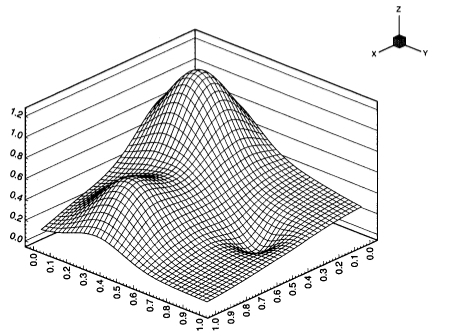
\includegraphics[scale=1.5]{CGOUT1.jpg}
\end{figure}
On a considéré des éléments finis rectangles $C^1$ de Bogner-Fox-Schmidt, et la formule de quadrature sur les patchs est $P_3$ sur des triangles, et on prend $\varepsilon=10^{-6}$.\\
Il n'y a pas de méthode mathématique pour optimiser le choix de ce paramètre : on utilise une validation croisée.\\
\begin{figure}[!h]
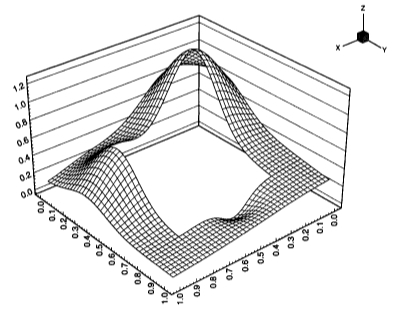
\includegraphics[scale=1.4]{CGOUT2.jpg}
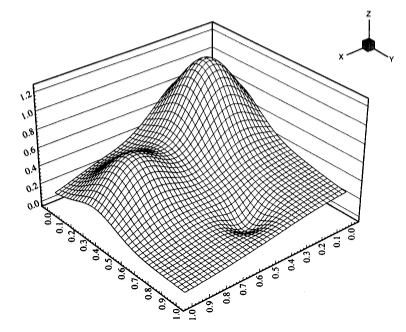
\includegraphics[scale=1.4]{CGOUT4.jpg}
\end{figure}
Comparaison des résultats avec une $D^m$-spline sur des données de Lagrange.\\
\end{block}
\end{column} %end column 2.1

\begin{column}{\onecolwid}\vspace{-.6in} % The second column within column 2 (column 2.2)
\begin{block}{Approximation numérique (2)}
\begin{figure}[!h]
\centering
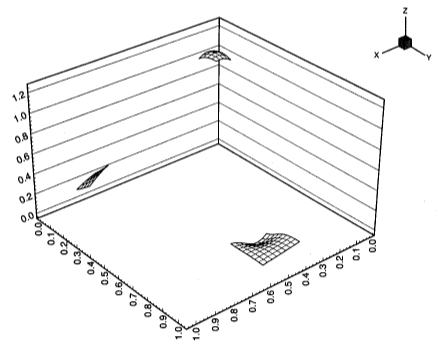
\includegraphics[scale=1.2]{CGOUT5.jpg}
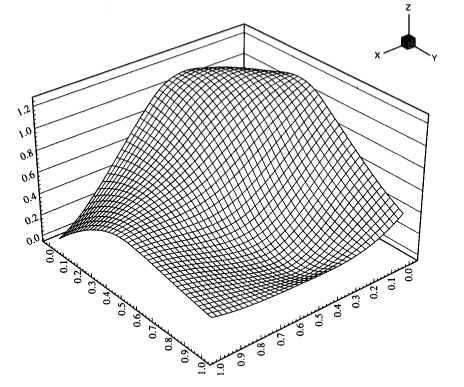
\includegraphics[scale=1.2]{CGOUT3.jpg}
\end{figure}
Calcul de l'erreur quadratique:
\[Q_{error}(\cup_{i}{(x_i,y_i,z_i))}=\frac{\sum_{i=1}^{1600}{(\tilde{z_i}-z_i)^2}}{\sum_{i=1}^{1600}{z_i^2}}) \]
\begin{center}
\begin{tabular}{|c|c|c|}
\hline
Fonction g & $Q_{error}$ & Data \\
\hline
Spline d'ajustement & $1.34\times10^{-3}$ & 1152 points \\
\hline
Spline d'ajustement & $0.18$ & 33 points \\
\hline
\end{tabular}
\end{center}

\bigskip
Exemple d'application réelle : Big Island à Hawaï. Plus de 7 000 points de données pour un relief allant de -4 à +4km. Les résultats sont affichés fig \ref{figBI}
\begin{figure}
\centering
\includegraphics[scale=0.8]{CGOUT6.png}
\caption{Approximation $C^1$, grille de 250$\times$250 points}
\label{figBI}
\end{figure}

\end{block}
\end{column} %end column 2.2

\end{columns} %end column split
\end{column} %end column with 2 columns

\begin{column}{\sepwid}\end{column} % Empty spacer column

\begin{column}{\onecolwid} % The third column


%----------------------------------------------------------------------------------------
%	REFERENCES
%----------------------------------------------------------------------------------------

\begin{block}{Réferences}

\nocite{*} % Insert publications even if they are not cited in the poster
\small{\bibliographystyle{unsrt}
\bibliography{bib}\vspace{0.75in}}

\end{block}

%----------------------------------------------------------------------------------------
%	CONTACT INFORMATION
%----------------------------------------------------------------------------------------

\setbeamercolor{block alerted title}{fg=black,bg=norange} % Change the alert block title colors
\setbeamercolor{block alerted body}{fg=black,bg=white} % Change the alert block body colors

\begin{alertblock}{Contact Information}

\begin{itemize}
\item Web: \href{http://lmi.insa-rouen.fr/}{http://lmi.insa-rouen.fr/}
\item Email: \href{mailto:christian.gout@insa-rouen.fr}{christian.gout@insa-rouen.fr}\\
 \href{mailto:conrad.hillairet@insa-rouen.fr}{conrad.hillairet@insa-rouen.fr}\\
 \href{mailto:alexandre.vieira@insa-rouen.fr}{alexandre.vieira@insa-rouen.fr}
\end{itemize}

\end{alertblock}

\begin{center}
\begin{tabular}{ccc}
\includegraphics[width=0.4\linewidth]{logo2.png} & \hfill & 
\includegraphics[width=0.6\linewidth]{logo.png}
\end{tabular}
\end{center}

\end{column} % End of the third column

\end{columns}
\end{frame}

\end{document}
